\documentclass{elsarticle}
\usepackage{amsmath}
\usepackage{graphicx}
\usepackage{hyperref}

\graphicspath{{figures/}}

% CASTEL PACKAGES
\usepackage{import}
\usepackage{xifthen}
\usepackage{pdfpages}
\usepackage{transparent}
% END CASTEL PACKAGES

\newcommand{\castelincfig}[2][1.0]{%
      \def\svgwidth{#1\columnwidth}
          \import{./figures/}{#2.pdf_tex}
          }

\newcommand{\todo}[1]{
  \textcolor{red}{\textbf{Todo}: #1}
}

%TITLE
\title{Moving domain formulation for AM of metals}
\author[1]{Mehdi Slimani}
\author[1]{Miguel Cervera}
\author[1]{Michele Chiumenti}
\affiliation[1]{organization={CIMNE}}
\date{\today}
%ETITLE

\begin{document}

\begin{abstract}
  This paper presents a framework to solve for
the thermal field in the partscale deposition
process in metallic Additive Manufacturing
using a Domain Decomposition approach.
Close to the laser, the heat equation is posed
in the reference
frame of the heat source,
and the rest of the domain is solved
for in the laboratory reference frame.
This work focuses on the temporal multiscale
nature of the problem. Notably, the constraint
of timestepping less than a radius per time step
is absent in this model. The steadiness
of the problem in the reference frame of the heat source
is taken advantage from in order to take bigger time steps
and time savings of around $\times 2-3$ are showcased
in an example case with deposition.

\end{abstract}

\maketitle

\section{Introduction}\label{sec:intro}
\todo{Additive manufacturing is cool}\par
\todo{However, simulation is slower than experiment}\par
\todo{Simulation is difficult because
is ``extremely multiscale'' \cite{Hodge2021}}\par
\todo{Time scale of radius and constraint on timestep}\par
\todo{Special techniques are required
\cite{Puso2023, Viguerie2022}}\par
\todo{Motivate new technique \cite{VanElsen2007, Mundra1996, Powar2016, Storti2022}}


\section{Description of methods}\label{sec:methodman}
\subsection{Brief description of reference model}
  In this work, the chosen reference model is
the following linear heat equation with convection
boundary conditions: solve for the temperature
field $T = f(x,t)$ such that

\begin{align}
  \rho c_p \partial_t T{\scriptstyle(x,t)} - \nabla \cdot (k \nabla T{\scriptstyle(x,t)}) &= r{\scriptstyle(x,t)}
  \qquad &\forall x &\in \Omega \label{eq:refheateq}\\
  q_{conv} &= h_{conv} ( T{\scriptstyle(x,t)} - T_{env} ) \qquad & \forall x &\in \partial \Omega {}_{conv}\notag
\end{align}

, where $\rho, \enskip c_p, \enskip k, \enskip  r, \enskip q_{conv} \textrm{ and } h_{conv}$
denote respectively
the density, the specific heat, the conductivity, volumetric
heat source, the convection heat flux and the convection coefficient.
The heat source adopted in this work is a standard Gaussian source:

\begin{equation}\label{eq:heatsource}
  r(\mathbf{x}, t) = \frac{6 \sqrt{3} P}{ \pi^{3/2} R^3}
  \exp\bigg( \frac{-3||\mathbf{x} - \mathbf{x_{hs}}||_2^2}{R^2}\bigg)
\end{equation}

, where $P, \enskip R \textrm{ and } \mathbf{x_{hs}}$
denote respectively the power, the radius and the position
of the heat source.\par

The time dependency of the domain is due to
the deposition
\footnote{ In the case of LPBF, this means that the powder is not modelled. }.
Numerically, this is modelled using  the born-dead element
technique \citep{Chiumenti2010}:
elements that are \textit{inactive} are not included in the
computational domain nor assembled,
and, at the beginning of each time step, a collision test
is performed with the geometry of the deposition
in order to \textit{activate} elements corresponding to
the newly deposited material.\par

Although this model misses important features like
thermal dependency of the parameters, radiation heat loss and
latent heat\citep{VanElsen2007, Hodge2021},
it has the advantage of being the simplest setting
where the proposed method can be illustrated.\par


\subsection{Proposed model}

Let us denote the change of reference frame by

$$
\mathbf{\xi} = \mathbf{x} - \int_0^t \mathbf{V}(t) dt
$$

, where $\mathbf{V} = f(t)$ denotes the
speed of the laser.
The proposed model is as follows:
in a \textit{moving} subdomain attached to the heat source,
$\Omega_m \subset \Omega$,
the problem is posed in the reference frame of the heat source.
In the remaining
\textit{fixed} subdomain $\Omega_f \subset \Omega$,
the problem is posed
in the usual laboratory reference frame.
The chosen domain decomposition framework is
a standard Neumann Dirichlet non-overlapping decomposition,
hence $\Omega_f = (\Omega \setminus \Omega_m)^{\mathrm{o}}$,
where ${}^{\mathrm{o}}$ denotes the interior of a set. Let
$\Gamma$ denote the interface between both subdomains,
$\Gamma = \partial \Omega_m \cap \partial \Omega_f$. In this
setting, system \ref{eq:refheateq} can be rewritten as

\begin{align}
  \rho c_p \Big( \partial_t T_m{\scriptstyle (\xi, t)} - \mathbf{V} \cdot \nabla T_m{\scriptstyle (\xi, t)} \Big) -
  \nabla \cdot ( k \nabla T_m{\scriptstyle (\xi, t)}) &= r{\scriptstyle (\xi)}  &\xi &\in \Omega_m \label{eq:pdeddm}\\
  k \partial_n T_m{\scriptstyle (\xi, t)} &= k \partial_n T_f  &\xi &\in \Gamma \notag\\
  q_{\textrm{conv}} &= h_{\textrm{conv}} ( T_m{\scriptstyle(\xi,t)} - T_{env} ) \qquad &\xi &\in \partial \Omega_{m, \textrm{conv}}\notag\\
  \rho c_p \partial_t T_f{\scriptstyle (x, t)} - \nabla \cdot (k \nabla T_f{\scriptstyle (x, t)}) &= r{\scriptstyle (x, t)} \qquad &x &\in \Omega_f \label{eq:pdedf}\\
  T_f{\scriptstyle (x, t)} &= T_m \qquad &x &\in \Gamma \notag\\
  q_{\textrm{conv}} &= h_{\textrm{conv}} ( T_f{\scriptstyle(x,t)} - T_{env} ) \qquad &x &\in \partial \Omega_{f, \textrm{conv}}\notag
\end{align}
, where $\mathbf{V}$ denotes the speed of the heat source. Note that
the time dependency of heat source is absent from \ref{eq:pdeddm}
Ideally, $\Omega_m$ is big enough
to contain the whole support of the heat source such that
the right hand side of \ref{eq:pdedf} is null.
\textit{Steamline Upwind Petrov Galerkin} stabilization is chosen
in order to take care of the newly introduced advection term
in \ref{eq:pdeddm}. The corresponding weak forms write respectively

\begin{align}
  \label{eq:weakformdm}
    \int_{\Omega_m} v_m \rho c_p \partial_t T_m 
  - \int_{\Omega_m} v_m \rho c_p \mathbf{V} \cdot \nabla T_m
  + \int_{\Omega_m} k \nabla v_m \cdot \nabla T_m&\\
  - \int_{\partial \Omega_{m, \textrm{conv}}} \hspace{-8mm} v_m \mathbf{q_{conv}} \cdot \hat{n}
  - \int_{\Gamma} k v_m \nabla T_f \cdot \hat{n} &\notag\\
  + \int_{\Omega_m} \tau r_h  \rho \mathbf{V} \cdot \nabla v_m &= \int_{\Omega_m} v_m r \notag\\
  \label{eq:weakformdf}
    \int_{\Omega_f} v_f \rho c_p \partial_t T_f 
  + \int_{\Omega_f} k \nabla v_f \cdot \nabla T_f
  - \int_{\partial \Omega_{f, \textrm{conv}}} \hspace{-8mm} v_f \mathbf{q_{conv}} \cdot \hat{n} &= \int_{\Omega_f} v_f r
\end{align}

, where $r_h$ is the residual of equation \ref{eq:pdeddm}.
For both this model and the reference, the spatial discretization
is carried out using P1/Q1 finite elements and Backward Euler
time integration. \cite{Puso2023} mentions that higher order
time integrations will introduce further oscillations.\par

% EXPLAIN MESHING
After discretization, the algebraic form obtained from
\ref{eq:weakformdm} and \ref{eq:weakformdf} writes as follows

\begin{equation}\label{eq:algebraic_coupled}
  \begin{bmatrix}
    \tilde{M} & \cdot \\
    \cdot & \tilde{M}
  \end{bmatrix}
\end{equation}

% EXPLAIN ASSEMBLY
\todo{Talk about geometrical operations}\par
\todo{Overview of timestep}\par

\begin{figure}
  \castelincfig{nonOverlappingPartition}
  \caption{Schematic of proposed model.}
  \label{fig:schematic}
\end{figure}


\iffalse
Show reference model
Go over limitations
Introduce my model
\fi


\section{Results}\label{sec:results}
The previously explained method was implemented
here: \url{https://github.com/ordinary-slim/moving_heat_source}.

\subsection{2D welding}

\begin{figure}[]
  \centering
  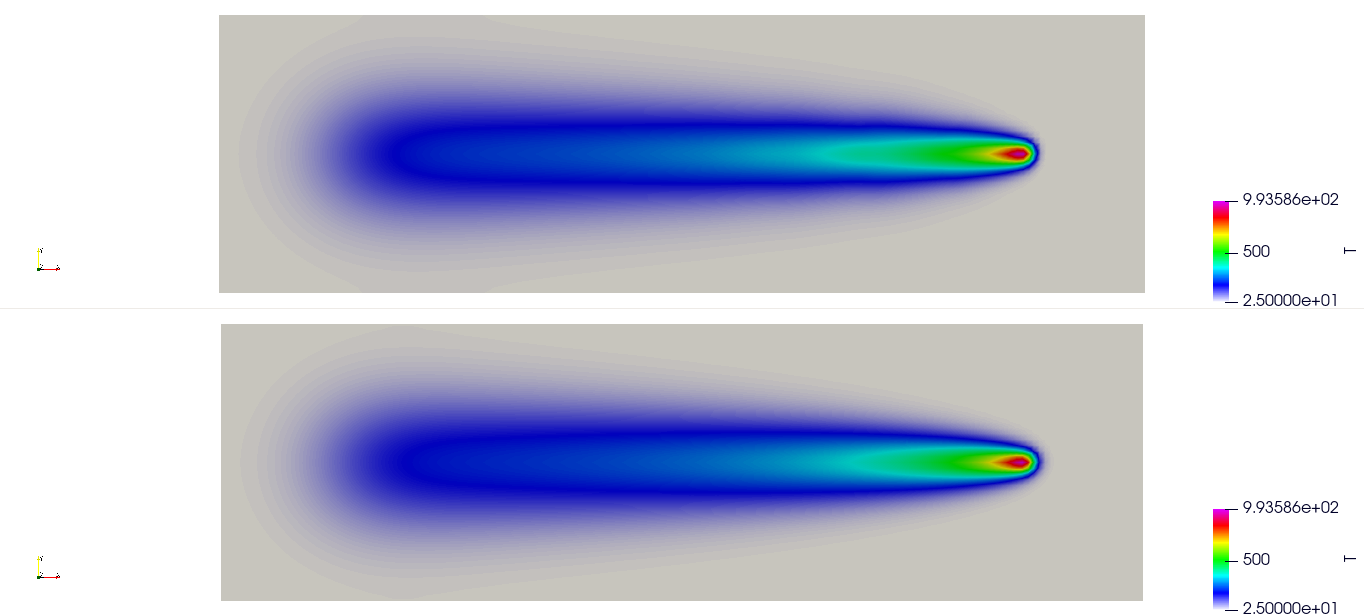
\includegraphics[width=\textwidth]{2d_welding/temptative.png}
  \caption{Top is mine, bottom is reference.}
  %\label{fig:meaningful label}
\end{figure}

\subsection{3D LPBF}

\begin{figure}[h]
  \centering
  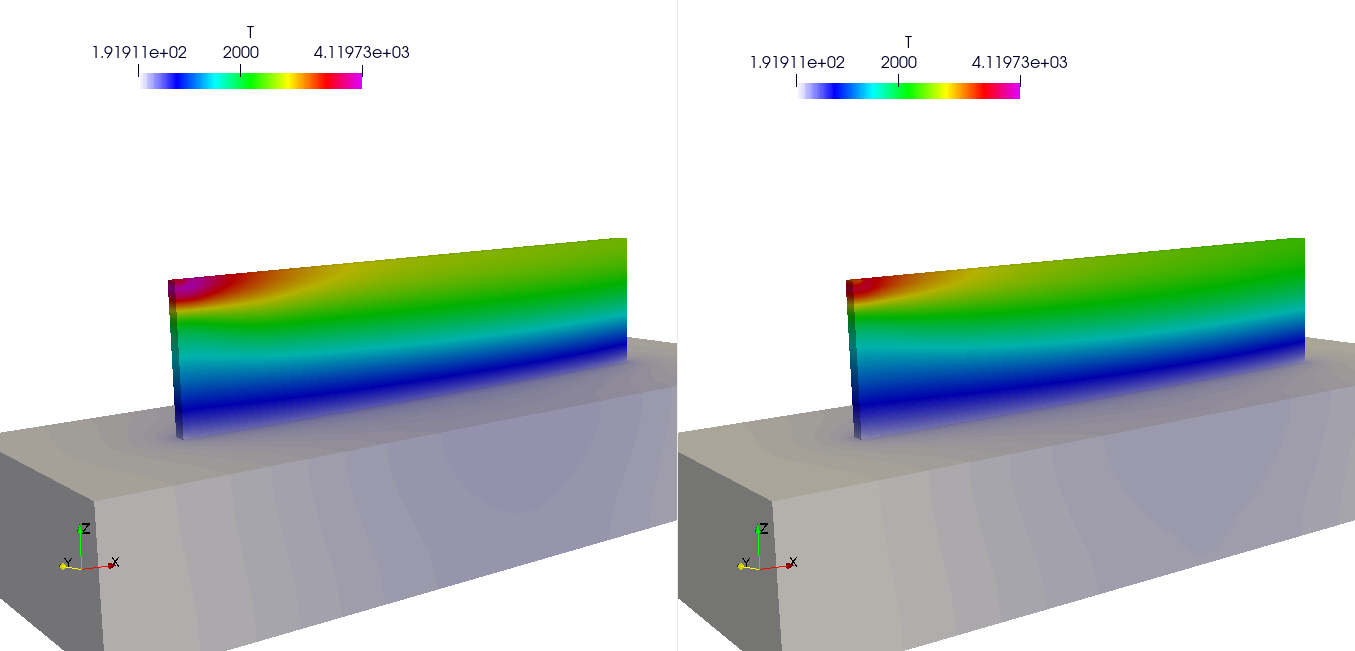
\includegraphics[width=\textwidth]{3d_lpbf/temptative.png}
  \caption{Top is mine, bottom is reference.}
  %\label{fig:meaningful label}
\end{figure}



\section{Conclusions}\label{sec:conclusions}
\begin{itemize}
  \item Proposed model allows some gain in terms
    of time steps.
  \item Proposed model might have some other gains
    that remain unexplored.
\end{itemize}


\bibliographystyle{plain}
\bibliography{refs}

\end{document}
